\section{Wind energy}
A brief investigation of wind energy showed that the \emph{mechanical rotor power} $P_{\mathrm R} = \mathrm{d} T_{\mathrm W}/\mathrm{d} t$ in $\left(\mathrm W \right)$ can be determinerd from the time derivative of the kinetic energy $T_{\mathrm W}$ in $\left(\mathrm{Wh} \right)$ of a flowing gas -- which makes up the atmosphere of a planet and is also known as wind -- with the \emph{mass} $m_{\mathrm {gas}}$ in $\left(\mathrm{kg} \right)$, the uniform and constant \emph{flow velocity} $v_{\mathrm W}$ in $\left(\mathrm{m} \mathrm{s^{-1}}\right)$, the \emph{density} near the ground\footnote{This only applies if the change in gas density at the height of the rotors of the wind turbine is negligible compared to the ground.} $\varrho_{\mathrm {gas}}$ in $\left(\mathrm{kg} \mathrm{m}^{-3}\right)$, the \emph{rotor radius} $r_{\mathrm{R}}$ in $\left(\mathrm{m}\right)$ and the \emph{performance coefficient}\footnote{Modern wind turbines reach a performance coefficient ranging from $0,35$ to $0,45$. According to Betz's law, the ideal perfomance coefficient is $0,5926$.} $c_{\mathrm P}$ in $\left( 1 \right)$. The area $A_\mathrm{W} = r_{\mathrm{R}}^2 \, \pi$ in $\left(\mathrm{m}^2 \right)$ must be perpendicular to the flowing gas. Taking into account the \emph{efficiency} of the mechanical transmission and the electrical generator $\eta_{\mathrm{mech}}$ in $\left( 1 \right)$, the \emph{generated electrical power} $P_{\mathrm{el}}$ in $\left(\mathrm W \right)$ can be calculated. A summary of this can be seen below \cite{Rebhan:2002, Flosdorff:2008, Hau:2016, Gawlik:2018}:
\begin{equation}
	\vcenter{\hbox{\begin{minipage}{.5\textwidth}
		\centering
		

\tikzset{every picture/.style={line width=0.75pt}} %set default line width to 0.75pt        

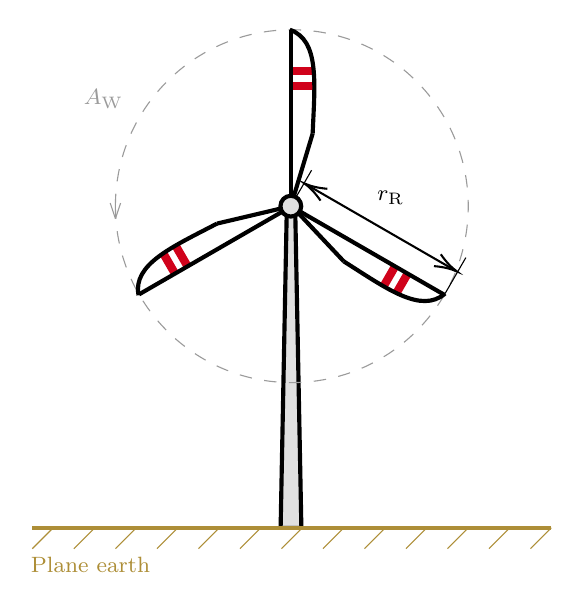
\begin{tikzpicture}[x=0.75pt,y=0.75pt,yscale=-1,xscale=1]
%uncomment if require: \path (0,345); %set diagram left start at 0, and has height of 345

%Straight Lines [id:da2855457278708555] 
\draw    (154.52,97.68) -- (144.52,115) ;
%Shape: Trapezoid [id:dp6563165495841363] 
\draw  [fill={rgb, 255:red, 224; green, 224; blue, 224 }  ,fill opacity=1 ][line width=1.5]  (139.6,270) -- (142.6,115) -- (146.6,115) -- (149.6,270) -- cycle ;
%Shape: Circle [id:dp4391264400751236] 
\draw  [color={rgb, 255:red, 155; green, 155; blue, 155 }  ,draw opacity=1 ][dash pattern={on 4.5pt off 4.5pt}] (60,115) .. controls (60,68.06) and (98.06,30) .. (145,30) .. controls (191.94,30) and (230,68.06) .. (230,115) .. controls (230,161.94) and (191.94,200) .. (145,200) .. controls (98.06,200) and (60,161.94) .. (60,115) -- cycle ;
%Straight Lines [id:da2732716340606678] 
\draw [color={rgb, 255:red, 208; green, 2; blue, 27 }  ,draw opacity=1 ][line width=3]    (144.52,50) -- (155.52,50) ;
%Straight Lines [id:da3625566257672834] 
\draw [color={rgb, 255:red, 208; green, 2; blue, 27 }  ,draw opacity=1 ][line width=3]    (144.52,57) -- (155.52,57) ;
%Straight Lines [id:da3551490622606075] 
\draw [line width=1.5]    (144.52,30) -- (144.52,115) ;
%Curve Lines [id:da31858770163213945] 
\draw [line width=1.5]    (144.04,30) .. controls (158.54,35) and (156.02,56) .. (155.04,80) ;
%Straight Lines [id:da40134971489014015] 
\draw [line width=1.5]    (144.52,115) -- (155.04,80) ;
%Straight Lines [id:da6221475193546597] 
\draw [color={rgb, 255:red, 208; green, 2; blue, 27 }  ,draw opacity=1 ][line width=3]    (194.75,144) -- (189.25,153.53) ;
%Straight Lines [id:da46600729912444394] 
\draw [color={rgb, 255:red, 208; green, 2; blue, 27 }  ,draw opacity=1 ][line width=3]    (200.81,147.5) -- (195.31,157.03) ;
%Straight Lines [id:da24248073534191383] 
\draw [line width=1.5]    (218.13,157.5) -- (144.52,115) ;
%Curve Lines [id:da8105786474721348] 
\draw [line width=1.5]    (218.85,157.08) .. controls (207.27,167.14) and (190.35,154.46) .. (170.05,141.61) ;
%Straight Lines [id:da649738591055431] 
\draw [line width=1.5]    (145,115) -- (170.05,141.61) ;
%Straight Lines [id:da39570308318736713] 
\draw [color={rgb, 255:red, 208; green, 2; blue, 27 }  ,draw opacity=1 ][line width=3]    (88.71,147.5) -- (83.21,137.97) ;
%Straight Lines [id:da21160602066475165] 
\draw [color={rgb, 255:red, 208; green, 2; blue, 27 }  ,draw opacity=1 ][line width=3]    (94.77,144) -- (89.27,134.47) ;
%Straight Lines [id:da9797525004071665] 
\draw [line width=1.5]    (71.39,157.5) -- (145,115) ;
%Curve Lines [id:da9490200570005278] 
\draw [line width=1.5]    (71.15,157.92) .. controls (68.23,142.86) and (87.67,134.54) .. (108.95,123.39) ;
%Straight Lines [id:da6466154668803934] 
\draw [line width=1.5]    (144.52,115) -- (108.95,123.39) ;
%Shape: Circle [id:dp4546700879564365] 
\draw  [fill={rgb, 255:red, 224; green, 224; blue, 224 }  ,fill opacity=1 ][line width=1.5]  (139.52,115) .. controls (139.52,112.24) and (141.76,110) .. (144.52,110) .. controls (147.28,110) and (149.52,112.24) .. (149.52,115) .. controls (149.52,117.76) and (147.28,120) .. (144.52,120) .. controls (141.76,120) and (139.52,117.76) .. (139.52,115) -- cycle ;
%Straight Lines [id:da5512625411833432] 
\draw [color={rgb, 255:red, 173; green, 142; blue, 55 }  ,draw opacity=1 ][fill={rgb, 255:red, 139; green, 87; blue, 42 }  ,fill opacity=1 ][line width=1.5]    (20,270) -- (270,270) ;
%Straight Lines [id:da5304059380179822] 
\draw [color={rgb, 255:red, 173; green, 142; blue, 55 }  ,draw opacity=1 ]   (50,270) -- (40,280) ;
%Straight Lines [id:da3431793884624006] 
\draw [color={rgb, 255:red, 173; green, 142; blue, 55 }  ,draw opacity=1 ]   (70,270) -- (60,280) ;
%Straight Lines [id:da7136874676914755] 
\draw [color={rgb, 255:red, 173; green, 142; blue, 55 }  ,draw opacity=1 ]   (30,270) -- (20,280) ;
%Straight Lines [id:da21878729454445067] 
\draw [color={rgb, 255:red, 173; green, 142; blue, 55 }  ,draw opacity=1 ]   (90,270) -- (80,280) ;
%Straight Lines [id:da2119530108548371] 
\draw [color={rgb, 255:red, 173; green, 142; blue, 55 }  ,draw opacity=1 ]   (110,270) -- (100,280) ;
%Straight Lines [id:da9669600696257283] 
\draw [color={rgb, 255:red, 173; green, 142; blue, 55 }  ,draw opacity=1 ]   (130,270) -- (120,280) ;
%Straight Lines [id:da148721087656281] 
\draw [color={rgb, 255:red, 173; green, 142; blue, 55 }  ,draw opacity=1 ]   (150,270) -- (140,280) ;
%Straight Lines [id:da021478871305470992] 
\draw [color={rgb, 255:red, 173; green, 142; blue, 55 }  ,draw opacity=1 ]   (170,270) -- (160,280) ;
%Straight Lines [id:da6475678117315542] 
\draw [color={rgb, 255:red, 173; green, 142; blue, 55 }  ,draw opacity=1 ]   (190,270) -- (180,280) ;
%Straight Lines [id:da17413992256591215] 
\draw [color={rgb, 255:red, 173; green, 142; blue, 55 }  ,draw opacity=1 ]   (210,270) -- (200,280) ;
%Straight Lines [id:da3680869151900985] 
\draw [color={rgb, 255:red, 173; green, 142; blue, 55 }  ,draw opacity=1 ]   (230,270) -- (220,280) ;
%Straight Lines [id:da19438567917294902] 
\draw [color={rgb, 255:red, 173; green, 142; blue, 55 }  ,draw opacity=1 ]   (250,270) -- (240,280) ;
%Straight Lines [id:da0327170377597672] 
\draw [line width=0.75]    (222.88,145.5) -- (152.73,105) ;
\draw [shift={(151,104)}, rotate = 390] [color={rgb, 255:red, 0; green, 0; blue, 0 }  ][line width=0.75]    (10.93,-3.29) .. controls (6.95,-1.4) and (3.31,-0.3) .. (0,0) .. controls (3.31,0.3) and (6.95,1.4) .. (10.93,3.29)   ;
\draw [shift={(224.61,146.5)}, rotate = 210] [color={rgb, 255:red, 0; green, 0; blue, 0 }  ][line width=0.75]    (10.93,-3.29) .. controls (6.95,-1.4) and (3.31,-0.3) .. (0,0) .. controls (3.31,0.3) and (6.95,1.4) .. (10.93,3.29)   ;
%Straight Lines [id:da7589968423979443] 
\draw    (228.85,139.76) -- (218.85,157.08) ;
%Straight Lines [id:da015160365704311562] 
\draw [color={rgb, 255:red, 155; green, 155; blue, 155 }  ,draw opacity=1 ]   (60,121) -- (57.5,113.5) ;
%Straight Lines [id:da4975603923384009] 
\draw [color={rgb, 255:red, 155; green, 155; blue, 155 }  ,draw opacity=1 ]   (60,121) -- (62.5,113.5) ;

%Straight Lines [id:da5866655581447886] 
\draw [color={rgb, 255:red, 173; green, 142; blue, 55 }  ,draw opacity=1 ]   (270,270) -- (260,280) ;

% Text Node
\draw (185,106.4) node [anchor=north west][inner sep=0.75pt]  [font=\footnotesize]  {$r_{\mathrm{R}}$};
% Text Node
\draw (18,283) node [anchor=north west][inner sep=0.75pt]  [font=\footnotesize,color={rgb, 255:red, 173; green, 142; blue, 55 }  ,opacity=1 ] [align=left] {Plane earth};
% Text Node
\draw (43.5,57.4) node [anchor=north west][inner sep=0.75pt]  [font=\footnotesize,color={rgb, 255:red, 155; green, 155; blue, 155 }  ,opacity=1 ]  {$A_{\mathrm{W}}$};


\end{tikzpicture}

		\captionof{figure}{Turbine that converts kinetic energy from wind into electrical energy. The dashed circle represents the area $A_\mathrm{W}$ that is perpendicular to a flowing gas.}
	\end{minipage}}}
	\qquad\qquad
		\begin{gathered}
		T_{\mathrm W} = \frac{1}{2} \, m_{\mathrm {gas}} \, v_{\mathrm W}^2 \text{,}
		\\
		\vdots
		\\
		\dfrac{\mathrm{d} T_{\mathrm W}}{\mathrm{d} t} = \frac{c_{\mathrm P}}{2} \, \varrho_{\mathrm {gas}} \, v_{\mathrm W}^3 \, \underbrace{\pi \, r_{\mathrm{R}}^2}_{A_\mathrm{W}} \text{,}
		\\
		P_{\mathrm{el}} = \eta_{\mathrm{mech}} \, \dfrac{\mathrm{d} T_{\mathrm W}}{\mathrm{d} t} \text{.}
	\end{gathered}
\end{equation}

This method of converting electrical energy however, was rejected mainly due to the unpredictability of $v_{\mathrm W}$.\footnote{The direction from which the wind comes is irrelevant for most small-scale wind turbines, as they are rotatably mounted on a mast.} In order to bridge times when no wind blows, a large energy storage device would have to be required, which would be charged in times of strong wind. But due to the high acquisition costs of a large energy storage devices, and the relative short duration of the OeWF's missions, this approach is not practical. Another important aspect that led to the rejection of this method is the fact that mean wind speeds are highly dependent on the location and in most parts of the world, $10 \mathrm m$ above the ground, these are usually between $5 \mathrm m \mathrm s^{-1}$ to less than $2,5 \mathrm m \mathrm s^{-1}$ as shown in maps provided by \cite{Atlas:2020}. In addition it must be added, that the gas density of air on the Earth's surface $\varrho_{\mathrm {gas,E}} = 1,217 \mathrm{kg} \mathrm{m}^{-3}$ is a lot higher than the gas density on the Martian surface $\varrho_{\mathrm {gas,M}} \approx 0,020 \mathrm{kg}  \mathrm{m}^{-3}$ -- which is mainly made up of carbon dioxide $\left( \mathrm{CO}_2 \right)$ -- and that the wind speeds on Mars, measured by NASA's Viking Landers VL1 and VL2, range from $2 \mathrm m  \mathrm s^{-1}$ to $7 \mathrm m \mathrm s^{-1}$ during summer, $5 \mathrm m \mathrm s^{-1}$ to $10 \mathrm m \mathrm s^{-1}$ during fall and $17\mathrm m \mathrm s^{-1}$ to $30 \mathrm m  \mathrm s^{-1}$ during dust storms. It can therefore be seen that -- compared to Earth -- the greatest negative influnece on $P_{\mathrm R}$ is the density of the Martian atmosphere \cite{Grayzeck:2020, Williams:2020}.
